% =====================================================================
%  ECCV 2026 submission — formatted in the LNCS / ECCV style.
%  ECCV uses the Springer LNCS layout. This file compiles out-of-the-box
%  with the standard `llncs.cls` (TeX Live: texlive-publishers).
%  To use the official ECCV 2026 template, replace the \documentclass
%  line with `\documentclass[runningheads]{eccv2026}` and add the
%  eccv2026.sty / splncs04.bst files from the official kit; the body
%  below is template-agnostic.
%  Double-blind: author block is anonymized.
% =====================================================================
\documentclass[runningheads]{llncs}

\usepackage{graphicx}
\usepackage{booktabs}
\usepackage{amsmath}
\usepackage{array}
\usepackage{multirow}
\usepackage[table]{xcolor}
\usepackage{url}
\usepackage[hidelinks]{hyperref}

\renewcommand{\UrlFont}{\ttfamily\small}

\begin{document}

\title{Sequencing Technology Meets Assembler:\\ A Reproducible Low-Resource Benchmark of\\ Second- and Third-Generation Reads for\\ Small-Genome Assembly}

\titlerunning{A Low-Resource Multi-Generation Sequencing-Assembly Benchmark}

\author{Anonymous ECCV 2026 Submission}
\authorrunning{Anonymous ECCV 2026 Submission}
\institute{Paper ID \texttt{****}}

\maketitle

\begin{abstract}
Choosing a sequencing strategy under a fixed budget and modest compute
is a recurring decision in genomics, yet most comparisons conflate the
\emph{sequencing technology} with the \emph{assembly algorithm} and report
a single operating point. We present a reproducible, configuration-driven
benchmark that disentangles these factors for small-genome assembly. On the
\emph{Escherichia coli} K-12 MG1655 reference (4.64\,Mbp) we simulate four
read types---Illumina PE150, Oxford Nanopore R9 ($\sim$90\% identity) and
R10 ($\sim$99\%), and PacBio HiFi---across five coverage depths
(5--50$\times$) and assemble each with six tools (SPAdes, Flye, Raven,
miniasm, hifiasm, Unicycler), yielding 55 reference-grade assemblies scored
by reference-based (QUAST) and reference-free (BUSCO) metrics together with
wall-clock and peak-memory cost. Four findings emerge. (i) Short reads never
close the genome ($\geq$\,80 contigs even at 50$\times$), whereas every
long-read technology reaches a single contig by a \emph{minimum viable
coverage} of 20$\times$. (ii) Across the matrix the assembler explains as
much quality variance as the technology (0.25 vs.\ 0.24), so ``which
technology'' is under-specified without ``which assembler.'' (iii) A
cost--quality--compute Pareto analysis selects ONT~R10 at 20$\times$
(US\$0.92) as the budget-optimal strategy across all tested budgets.
(iv) Two reference-free / real-data tools---neural polishing (Medaka) and
$k$-mer QV (Merqury)---both underperform on simulated reads for the same
root cause, exposing a concrete limitation of simulation-only benchmarks.
All code, configs and seeds are released for one-command reproduction.
\keywords{genome assembly \and sequencing technologies \and benchmark
\and reproducibility \and Pareto analysis}
\end{abstract}

\section{Introduction}
De novo genome assembly reconstructs a genome from sequencing reads, and the
quality of the result depends jointly on the \emph{reads} (length, error
profile, depth) and the \emph{assembler} (de~Bruijn vs.\ overlap-based).
Practitioners with a fixed budget and a commodity workstation must decide
\emph{which sequencing technology}, \emph{at what depth}, with \emph{which
assembler}---a decision usually made from folklore rather than a controlled,
resource-aware comparison. Published comparisons typically (a) report one
coverage, (b) bind each technology to a single assembler, conflating the two
effects, and (c) evaluate only contiguity, ignoring cost and compute.

We address these gaps with a small-genome benchmark designed like a machine
learning benchmark: one ground-truth reference, several input data regimes,
a shared evaluation harness, and a controlled, factorial sweep. Our
contributions are:
\begin{enumerate}
\item A \textbf{configuration-driven, seed-fixed benchmark} (55 assemblies)
that varies technology, coverage, assembler and genome difficulty as
orthogonal axes, released for one-command reproduction.
\item A \textbf{technology-vs-assembler variance attribution} showing the two
factors contribute almost equally to assembly-quality variance.
\item A \textbf{cost--quality--compute Pareto analysis} with an explicit
\$/Gb model that yields a budget-driven recommendation and a
\emph{minimum viable coverage}.
\item A \textbf{repeat/plasmid stress test} and a \textbf{reference-free
evaluation audit}, plus an honest analysis of where \textbf{GPU neural
polishing} and \textbf{$k$-mer QV} fail on simulated data---a reusable
caution for simulation-based studies.
\end{enumerate}

\section{Related Work}
\textbf{Read simulators.} ART~\cite{art} models Illumina sequencing-by-synthesis
error; Badread~\cite{badread} simulates long reads with tunable length and
identity, enabling the controlled R9/R10/HiFi ``technology generations'' we
use. \textbf{Assemblers.} Short reads are assembled with de~Bruijn graph tools
such as SPAdes~\cite{spades}; long reads with overlap-layout-consensus and
repeat-graph tools such as miniasm~\cite{miniasm}, Raven~\cite{raven} and
Flye~\cite{flye}; HiFi with hifiasm~\cite{hifiasm}; and short+long hybrids with
Unicycler~\cite{unicycler}. \textbf{Evaluation.} QUAST~\cite{quast} provides
reference-based metrics (N50, genome fraction, mismatches/indels);
BUSCO~\cite{busco} and Merqury~\cite{merqury} provide reference-free
completeness and consensus-quality estimates; Medaka performs neural consensus
polishing of ONT assemblies. Modern long-read pipelines combine HiFi and ONT
\cite{verkko}. Unlike prior single-point comparisons, we treat technology and
assembler as separable factors and add a resource/cost dimension.

\section{Benchmark Design}
\label{sec:design}

\subsection{Reference genomes and synthetic stressors}
The base reference is \emph{E.\ coli} K-12 MG1655 (4.64\,Mbp), small enough to
run dozens of assemblies on a commodity machine. To probe \emph{repeat
resolution} and \emph{plasmid recovery}---the regimes where read length
matters most---we construct three synthetic variants: \texttt{rep\_v1} (a few
long tandem repeats), \texttt{rep\_v2} (multiple dispersed mid-length repeats),
and \texttt{plasmid} (a 50\,kbp circular replicon appended to the chromosome).

\subsection{Read simulation}
We simulate four technologies at five depths $\{5,10,20,30,50\}\times$ with a
fixed seed. Illumina PE150 reads use ART (HiSeq~2500 model). Long reads use
Badread with identity profiles encoding three generations:
ONT~R9 (mean $\approx$\,87--90\%), ONT~R10 ($\approx$\,99\%) and HiFi
($\approx$\,99.9\%). This isolates the effect of \emph{accuracy at fixed read
length}, i.e.\ the historical improvement trajectory of long-read sequencing.

\subsection{Assemblers}
Each technology is paired with the assemblers appropriate to it
(Table~\ref{tab:matrix}): SPAdes (Illumina); Flye, Raven and miniasm
(ONT~R9/R10); hifiasm and Flye (HiFi); Unicycler (Illumina+ONT hybrid).
Running \emph{multiple} assemblers per technology is what lets us separate the
technology effect from the tool effect.

\subsection{Evaluation and cost model}
Every assembly is scored with QUAST against the appropriate reference
(N50, \#contigs, genome fraction, mismatches/indels per 100\,kbp,
misassemblies) and with BUSCO (\texttt{bacteria\_odb10}, reference-free gene
completeness). We log peak RSS and wall-clock per run. A simple cost model
assigns a published \$/Gb to each technology; combined with the depth this
gives an estimated sequencing cost per configuration, enabling a
cost--quality--compute Pareto analysis.

\begin{table}[t]
\centering
\caption{Experiment matrix. L1 sweeps coverage$\times$assembler on the base
reference; L3 fixes 30$\times$ on the synthetic stressors. 55 assemblies in
total (46 L1 + 9 L3).}
\label{tab:matrix}
\begin{tabular}{lll}
\toprule
Axis & Values & \#\\
\midrule
Technology & Illumina, ONT~R9, ONT~R10, HiFi (+ hybrid) & 4(+1)\\
Coverage   & 5, 10, 20, 30, 50$\times$ & 5\\
Assembler  & SPAdes, Flye, Raven, miniasm, hifiasm, Unicycler & 6\\
Reference  & base, rep\_v1, rep\_v2, plasmid & 4\\
Evaluation & QUAST (ref) + BUSCO (ref-free) + RAM/time & ---\\
\bottomrule
\end{tabular}
\end{table}

\section{Experiments}
\label{sec:exp}

\subsection{Setup and reproducibility}
The pipeline is configuration-driven: a single \texttt{matrix.yaml} defines all
axes and a fixed seed set. Environments are provisioned reproducibly; all
tables and figures regenerate from the released scripts. Assemblies are
named by a canonical run-id \texttt{\{tech\}\_\{cov\}x\_\{assembler\}\_\{ref\}\_s\{seed\}},
which is the contract that lets the stages run independently.

\subsection{Contiguity vs.\ coverage: a minimum viable depth}
Table~\ref{tab:contigs} reports contig counts as a function of depth. Short
reads plateau at $\sim$80 contigs and \emph{never} close the genome, even at
50$\times$, reflecting their inability to span repeats. Every long-read
technology collapses to a single contig by 20$\times$; below that, assemblies
are fragmented. We therefore identify $20\times$ as the \emph{minimum viable
coverage} for closing this genome with long reads
(Fig.~\ref{fig:saturation}).

\begin{table}[t]
\centering
\caption{Number of contigs (lower is better) vs.\ coverage, one representative
assembler per technology (Illumina:SPAdes, ONT:Flye, HiFi:hifiasm,
Hybrid:Unicycler). Long reads close the genome at 20$\times$; short reads
never do.}
\label{tab:contigs}
\begin{tabular}{rrrrrr}
\toprule
Cov.\ ($\times$) & Illumina & ONT~R9 & ONT~R10 & HiFi & Hybrid\\
\midrule
5  & 1296 & 43 & 48 & 46 & 59\\
10 & 129  & 19 & 8  & 6  & 7\\
20 & 89   & 2  & \textbf{1} & \textbf{1} & \textbf{1}\\
30 & 82   & 2  & 2  & \textbf{1} & \textbf{1}\\
50 & 87   & 2  & \textbf{1} & \textbf{1} & \textbf{1}\\
\bottomrule
\end{tabular}
\end{table}

\begin{figure}[t]
\centering
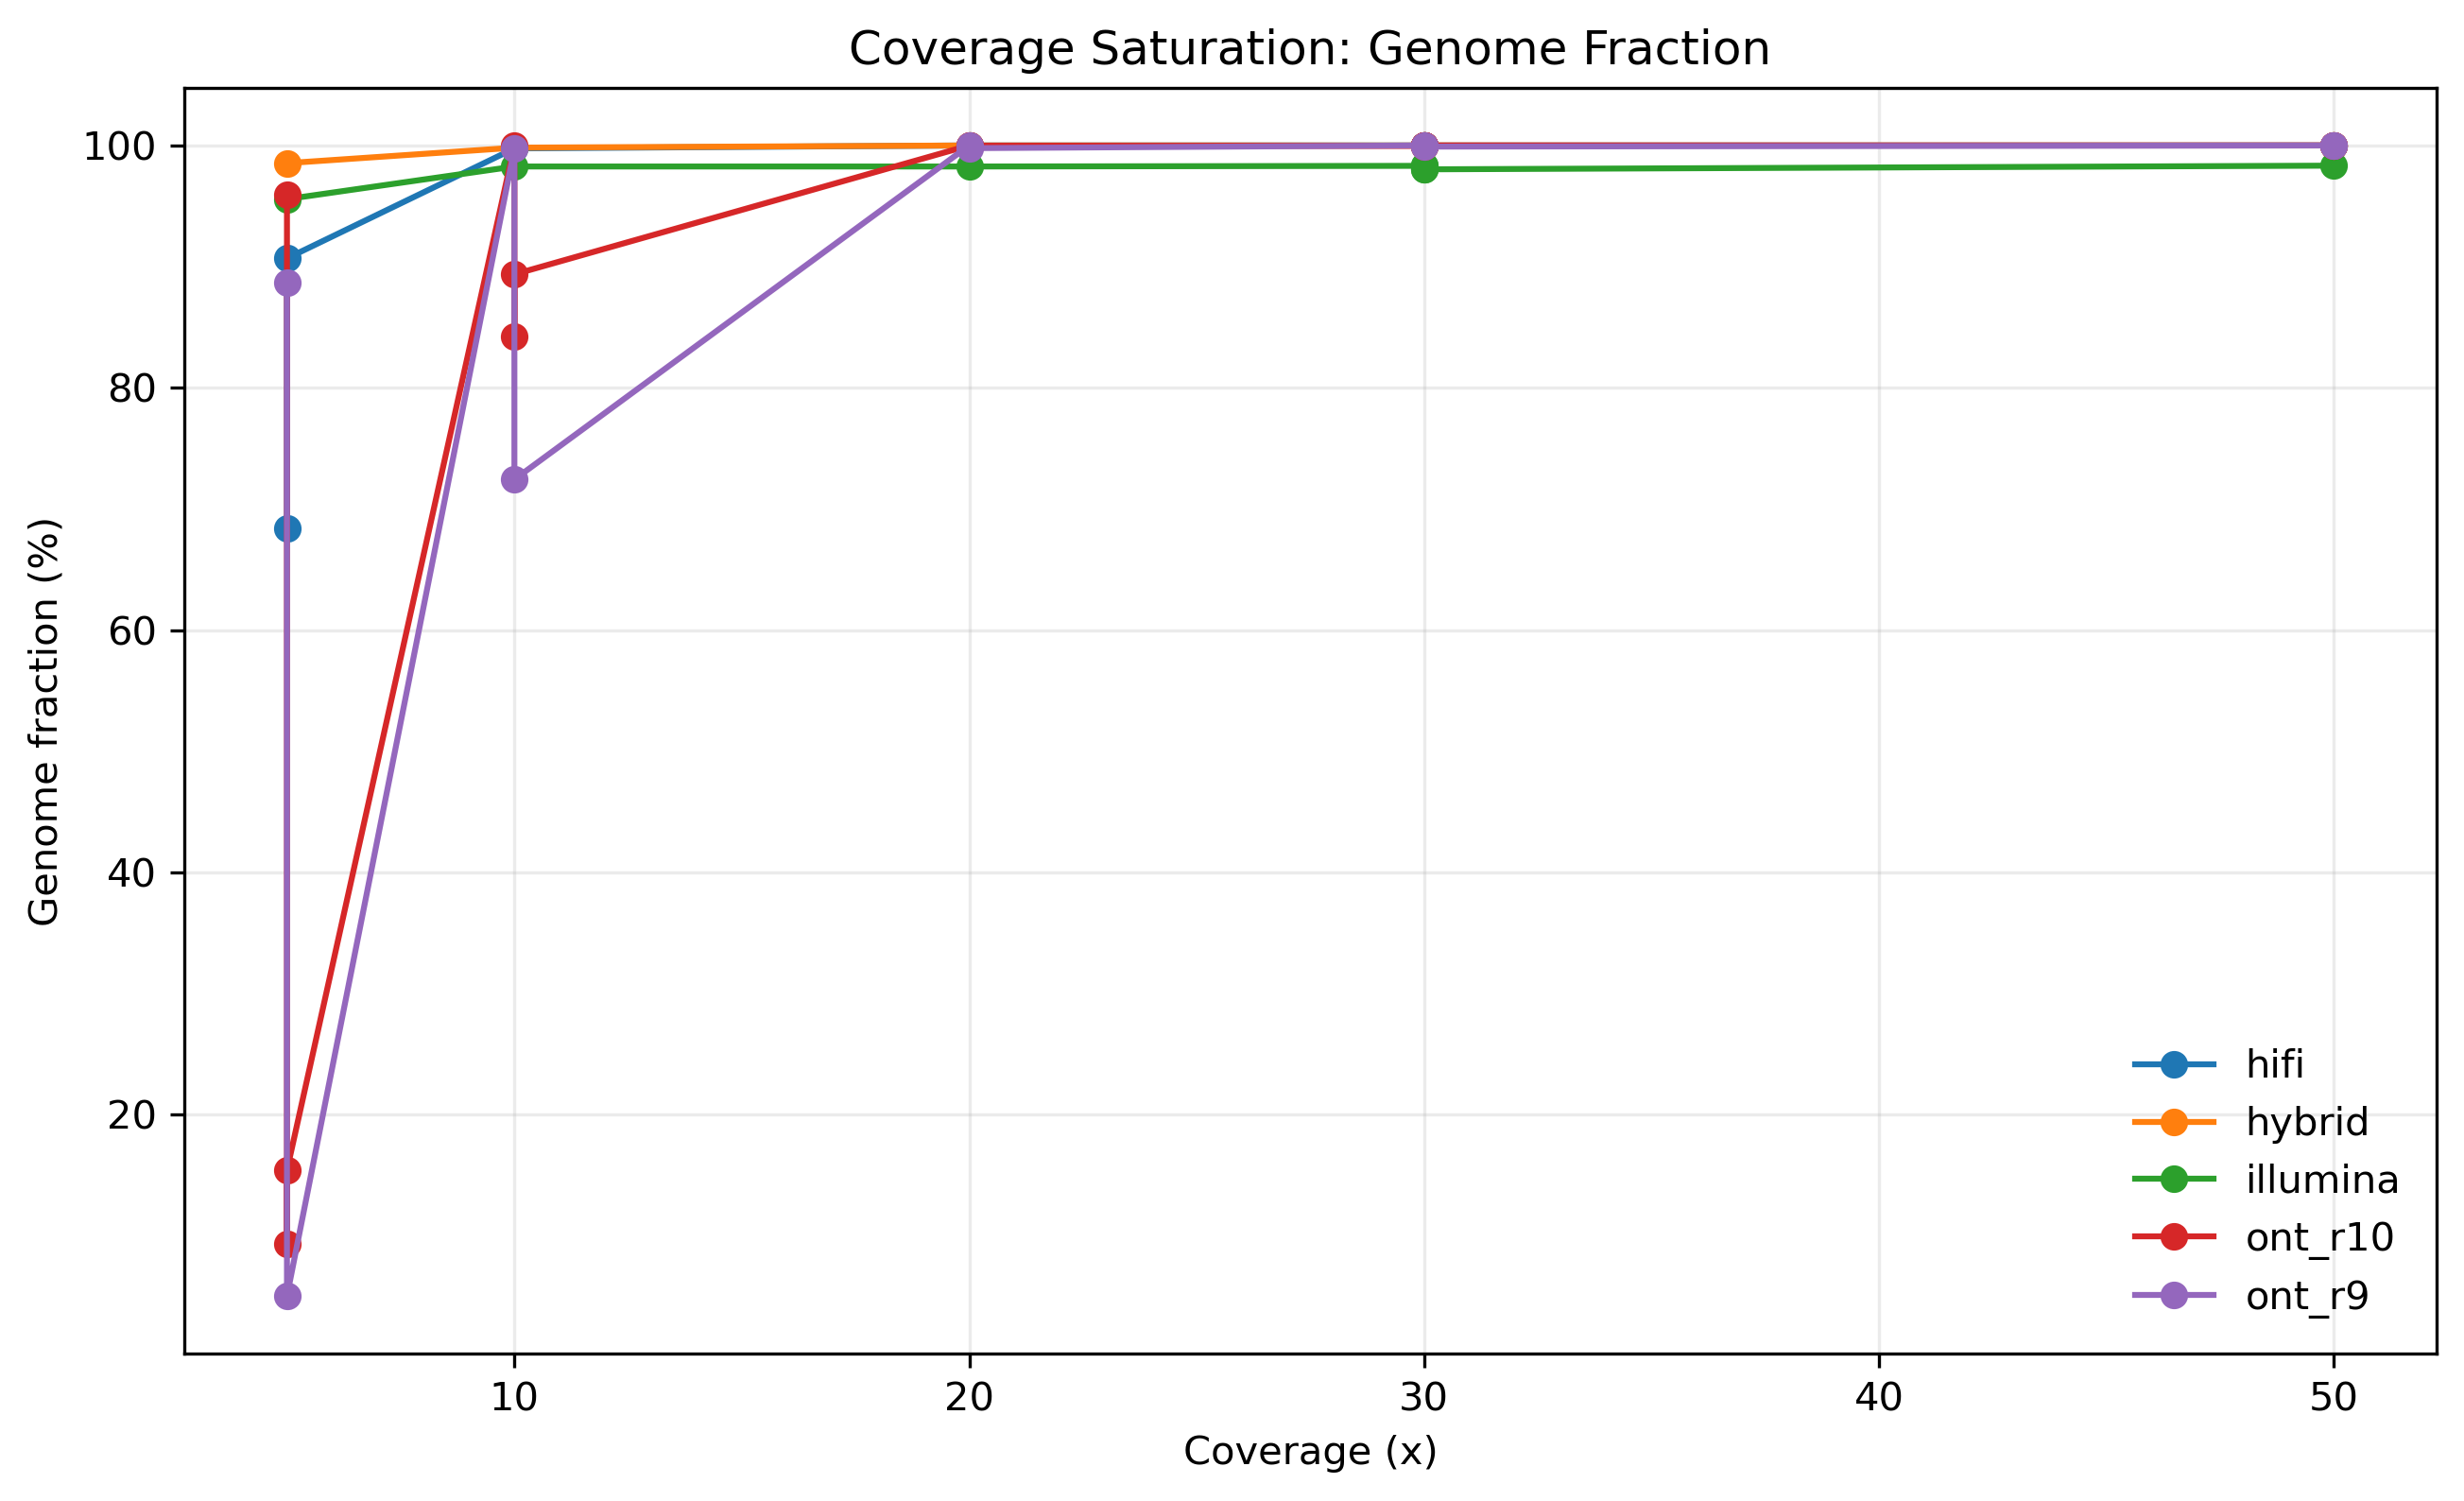
\includegraphics[width=0.62\linewidth]{figures/coverage_genome_fraction_curve.png}
\caption{Genome fraction vs.\ coverage. Long-read technologies saturate near
100\% by 20$\times$; short reads approach but do not complete the genome.}
\label{fig:saturation}
\end{figure}

\subsection{Technology vs.\ assembler: variance attribution}
A central question is how much of the quality difference is due to the
\emph{data} and how much to the \emph{tool}. Computing the between-group
variance share of N50 over the L1 matrix attributes
$0.239$ to technology and $0.249$ to assembler---\emph{nearly equal}. The
effect is vivid at low depth: ONT~R10 at 10$\times$ yields 8 contigs with Flye
but 44 and 51 with Raven and miniasm respectively. The tool can matter more
than a coverage step, so reporting a technology without its assembler is
under-specified.

\subsection{Generation effect: R9 $\rightarrow$ R10}
Holding read length fixed and varying only identity isolates the
``third-generation is not monolithic'' effect. ONT~R10 reaches a single contig
at 20$\times$ and remains near zero indels, whereas ONT~R9 stalls at two
contigs through 30$\times$ and carries substantially higher indel rates
(e.g.\ 79.7 vs.\ 0.0 indels/100\,kbp at 30$\times$). Modern ONT accuracy thus
closes most of the gap to HiFi on this genome.

\subsection{Cost--quality--compute Pareto}
Combining quality, the \$/Gb cost model and measured compute, the
budget-optimal configuration that achieves $\geq$99\% genome fraction with a
single contig is \textbf{ONT~R10 at 20$\times$ with Flye}, at an estimated
US\$0.92 and a peak memory well within a commodity machine. This choice is
stable across budgets from US\$1 to US\$20: once the Pareto-optimal knee is
reached, additional spend buys nothing (Fig.~\ref{fig:pareto}). Assembly
compute is minor---41 assemblies total $\approx$31\,min of wall time---so the
practical bottleneck is sequencing cost and read simulation, not assembly.

\begin{figure}[t]
\centering
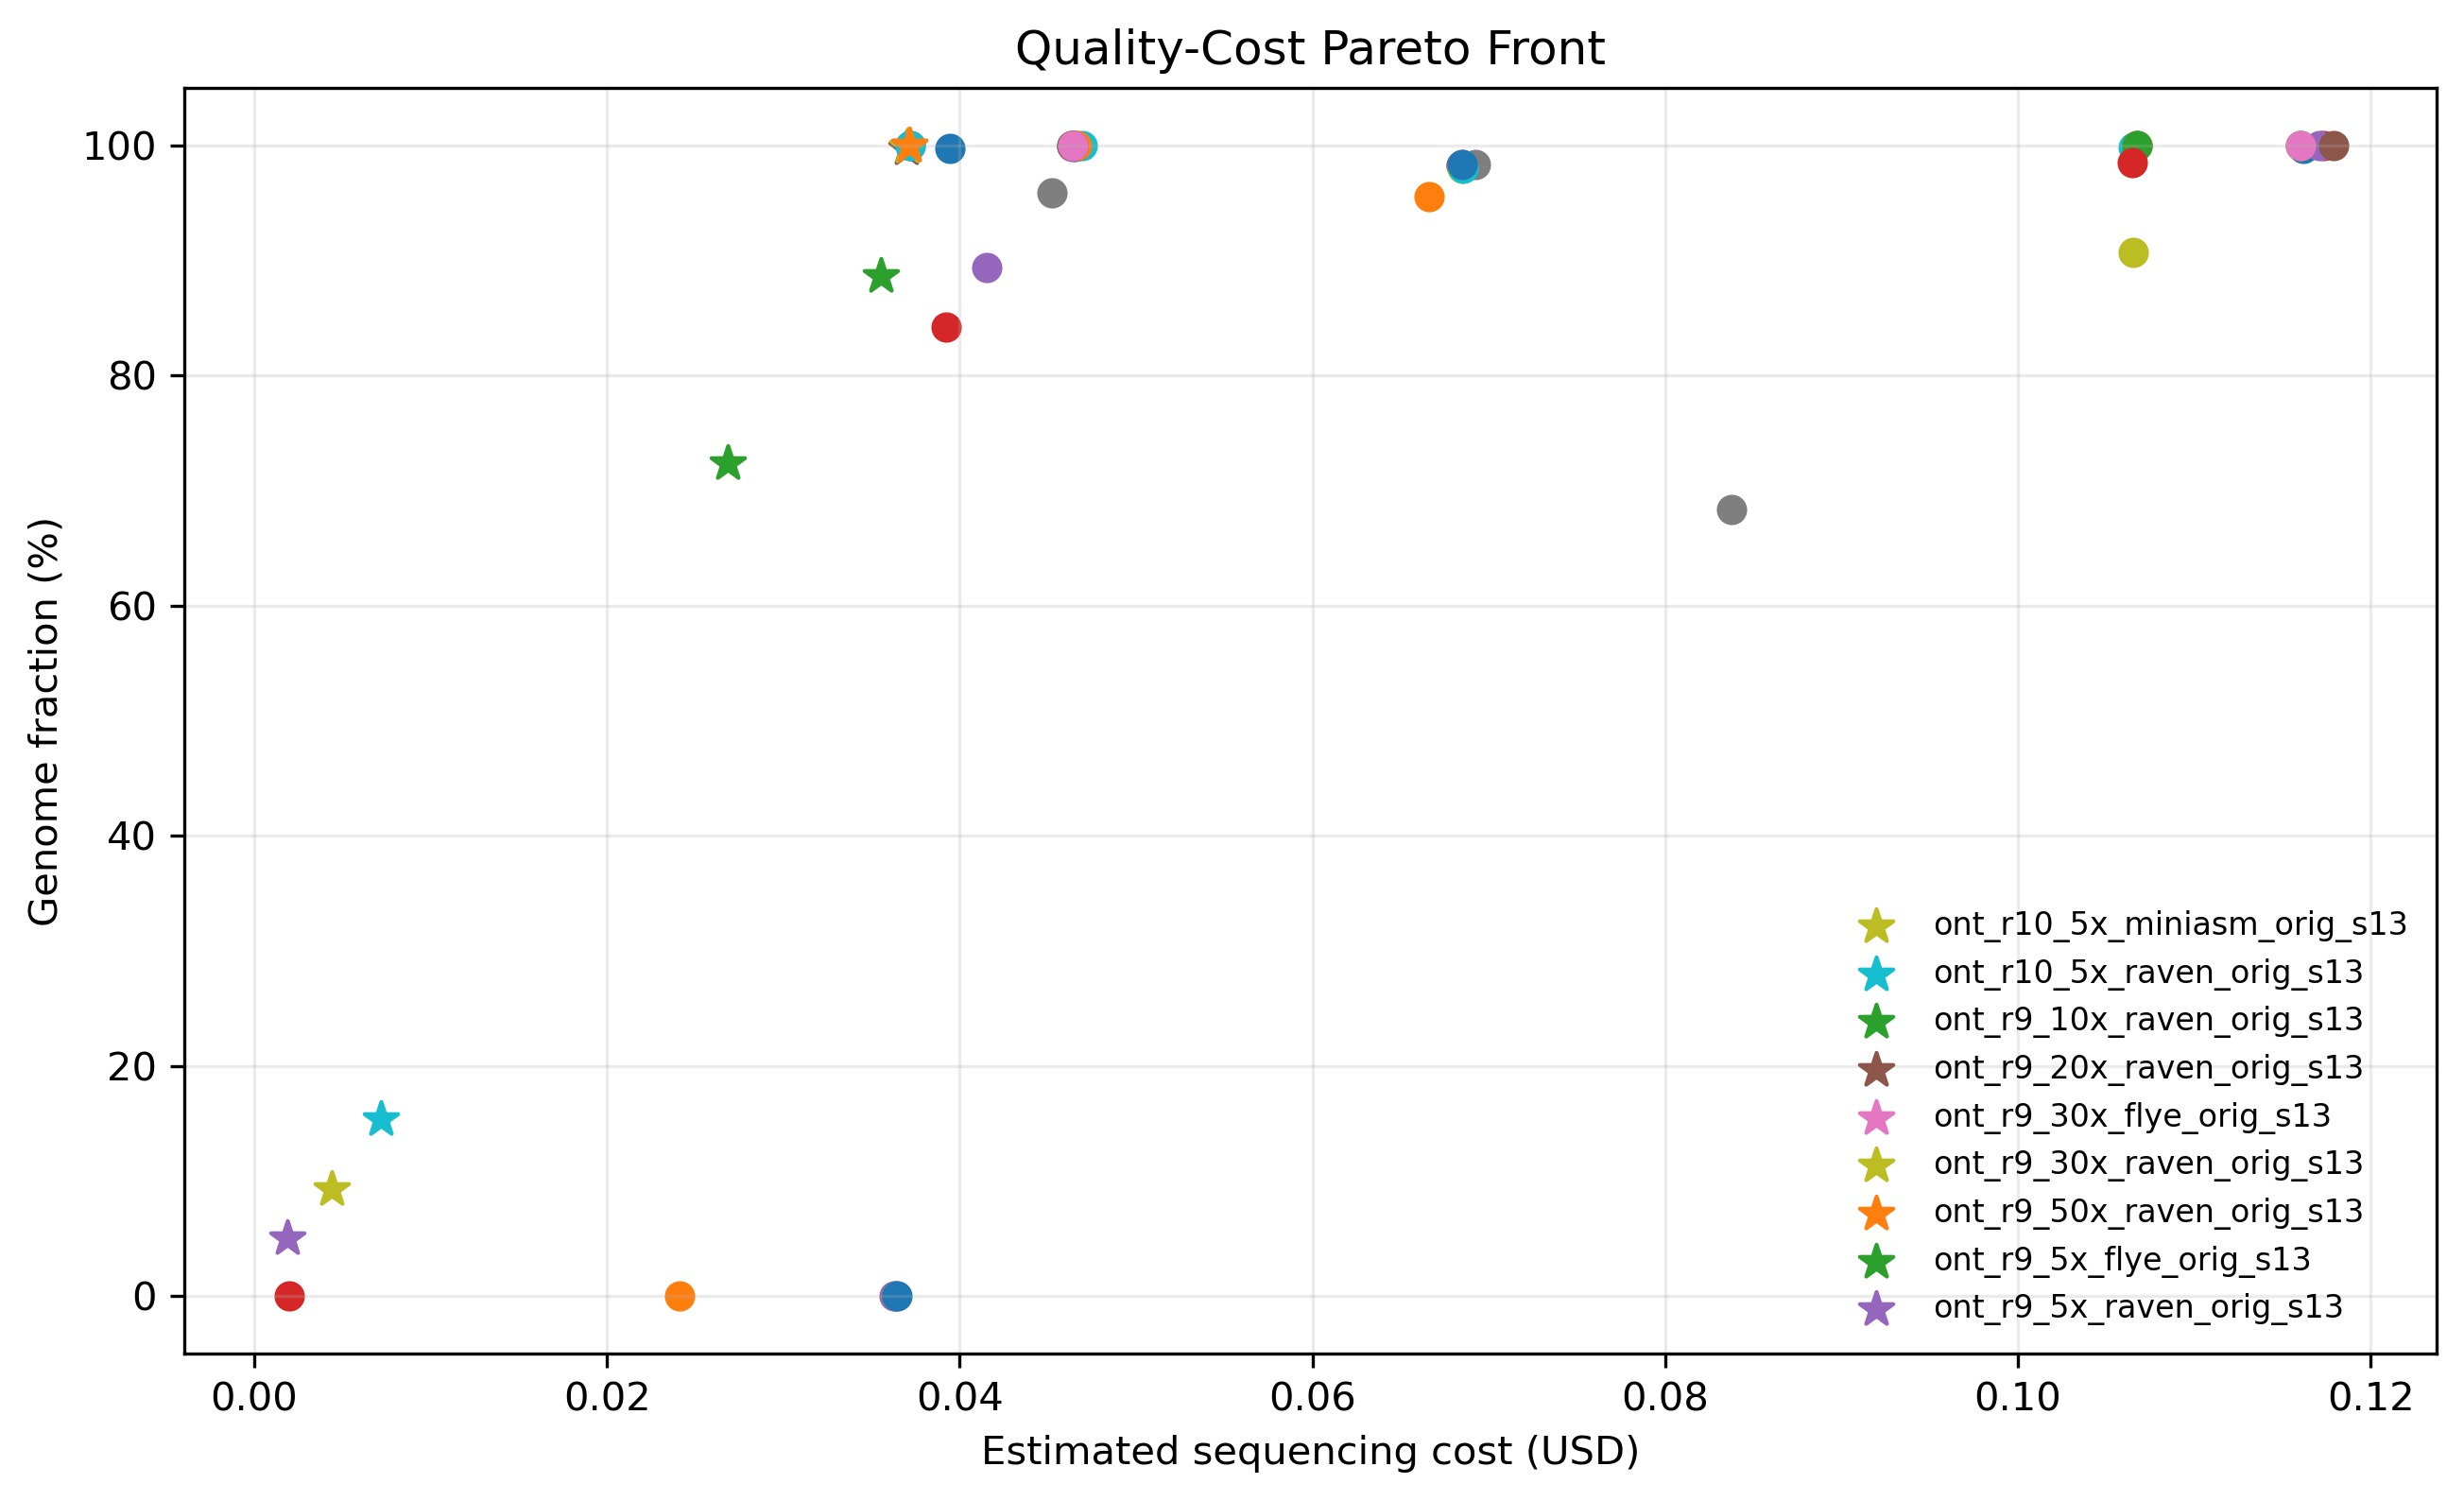
\includegraphics[width=0.6\linewidth]{figures/pareto_quality_cost.png}
\caption{Cost--quality Pareto front. The knee (ONT~R10, 20$\times$) dominates;
higher-cost points do not improve completeness.}
\label{fig:pareto}
\end{figure}

\subsection{Repeat and plasmid stress (L3)}
On the synthetic stressors at 30$\times$ (Table~\ref{tab:l3}), short reads stay
at 80+ contigs and miss structure, while ONT~R10 and HiFi recover the genome to
1--3 contigs at near-100\% genome fraction, including the plasmid. This
demonstrates the \emph{mechanism} behind the long-read advantage---spanning
repeats and recovering small replicons---rather than only its outcome.

\begin{table}[t]
\centering
\caption{Repeat/plasmid stress test at 30$\times$ (contigs / genome fraction \%).
Short reads fragment; long reads resolve.}
\label{tab:l3}
\begin{tabular}{lccc}
\toprule
Reference & Illumina (SPAdes) & ONT~R10 (Flye) & HiFi (hifiasm)\\
\midrule
rep\_v1  & 87 / 98.0 & 2 / 99.9 & 2 / 100\\
rep\_v2  & 91 / 98.0 & 1 / 100  & 3 / 100\\
plasmid  & 83 / 98.3 & 2 / 100  & 2 / 100\\
\bottomrule
\end{tabular}
\end{table}

\subsection{Reference-free evaluation and audit}
Reference-free metrics matter because real projects lack a ground truth. BUSCO
gene completeness is available for all 55 assemblies and tracks genome fraction
in aggregate, but a rank-correlation \emph{audit} reveals only a moderate
agreement with reference-based quality (Spearman $\rho=0.48$ vs.\ genome
fraction, $0.57$ vs.\ N50; top-10 overlap 3/10). The reason is that on a
bacterium BUSCO saturates to 100\% complete even for fragmented assemblies, so
it reliably rejects \emph{bad} assemblies but cannot rank \emph{good} ones.
Reference-free completeness is thus a useful filter, not a replacement for
reference-based or structural metrics.

\subsection{GPU neural polishing: a simulation limitation}
We applied GPU neural polishing (Medaka, on an RTX~4090) to all ONT Flye
assemblies. Contrary to the usual expectation that polishing closes the
ONT$\rightarrow$HiFi accuracy gap, improvement on our \emph{simulated} reads is
negligible and, for R9, mismatches slightly \emph{increase}
(Fig.~\ref{fig:polish}; e.g.\ R9 30$\times$ mismatches 16.8$\rightarrow$26.7
per 100\,kbp). The cause is twofold: Medaka's neural model is trained on the
error statistics of \emph{real} ONT signal, which differ from the simulator's,
and the bundled R10 model is mismatched to R9 data. Independently, Merqury QV
could not be computed because simulated reads yield a degenerate $k$-mer
spectrum. Two real-data tools failing for the \emph{same} reason is a concrete,
generalizable caution: simulation-only benchmarks cannot evaluate methods that
learned from real sequencing noise.

\begin{figure}[t]
\centering
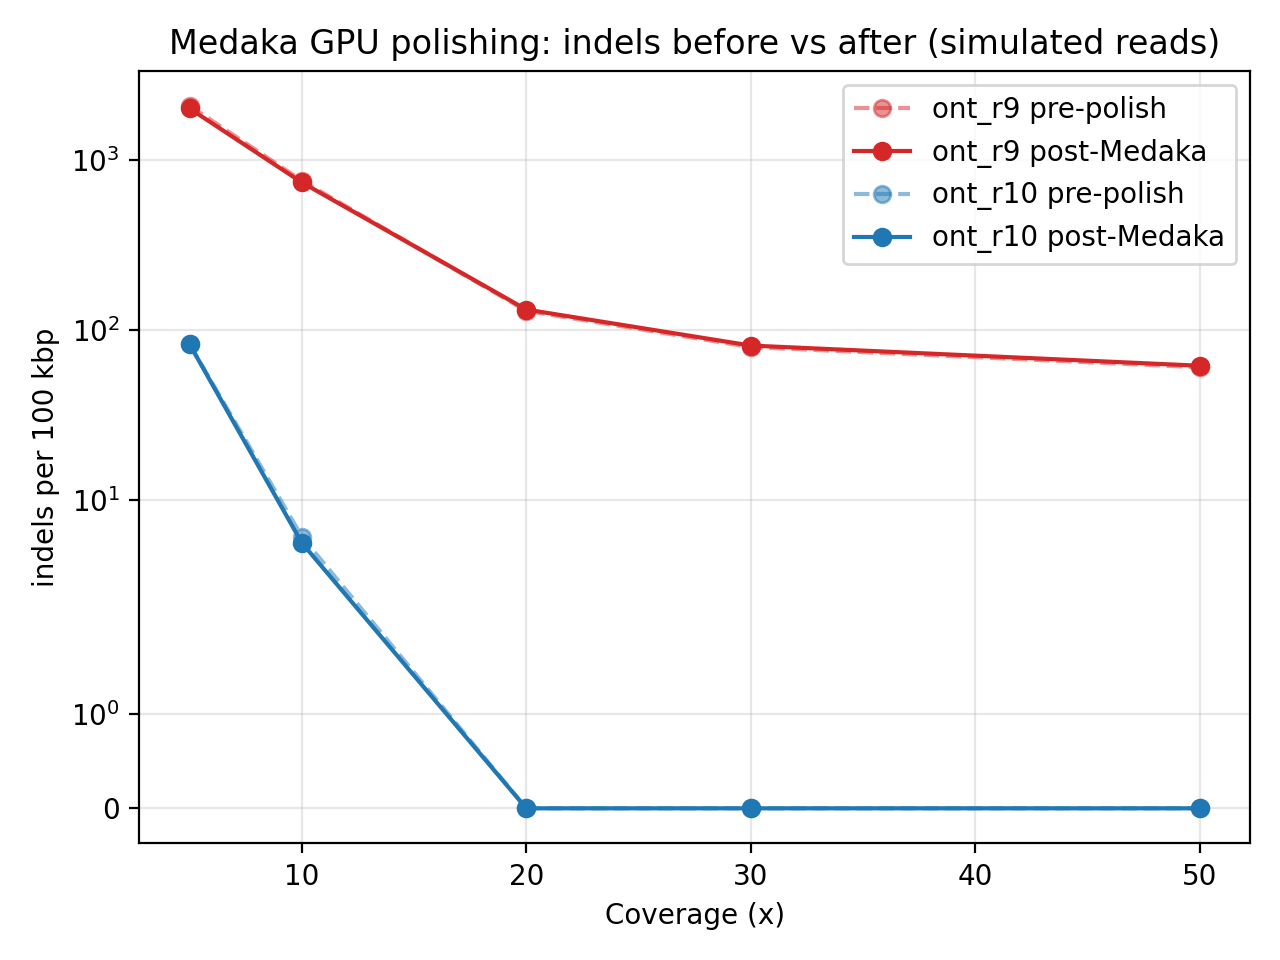
\includegraphics[width=0.6\linewidth]{figures/polish_indel_comparison.png}
\caption{Indels per 100\,kbp before vs.\ after Medaka polishing on simulated
ONT reads. Polishing barely moves the curves; R10 is already near-perfect by
20$\times$.}
\label{fig:polish}
\end{figure}

\subsection{Downstream gene recovery}
To test ``high N50 $\neq$ usable,'' we annotate representative assemblies with
Prokka and compare predicted features to the annotated reference
(Table~\ref{tab:downstream}). HiFi, ONT~R10 and the hybrid recover the full
complement (4302--4310 CDS, all 22 rRNA, 88 tRNA) in 1--2 contigs. The
fragmented short-read assembly (139 contigs) recovers fewer CDS (4235) and,
strikingly, only \textbf{14 of 22 rRNA genes}: ribosomal RNA operons are
repeats that short reads collapse, so contig fragmentation \emph{directly}
deletes biologically important genes. Contiguity therefore propagates into
downstream usability, not just summary statistics.

\begin{table}[t]
\centering
\caption{Downstream annotation (Prokka) at 30$\times$ vs.\ the reference. Short
reads lose rRNA operons (a repeat family) and truncate CDS.}
\label{tab:downstream}
\begin{tabular}{lrrrr}
\toprule
Assembly & Contigs & CDS & rRNA & tRNA\\
\midrule
Reference (truth)     & 1   & 4305 & 22 & 88\\
HiFi (hifiasm)        & 1   & 4302 & 22 & 88\\
ONT~R10 (Flye)        & 2   & 4310 & 22 & 88\\
Hybrid (Unicycler)    & 1   & 4305 & 22 & 88\\
Illumina (SPAdes)     & 139 & 4235 & \textbf{14} & 83\\
\bottomrule
\end{tabular}
\end{table}

\section{Discussion and Limitations}
Our study is deliberately scoped to a single small genome and to
\emph{simulated} reads, which makes it reproducible and low-cost but bounds its
external validity. The polishing and QV results above are precisely where
simulation breaks down, and motivate the clearest line of future work:
validate the recommendations on real ONT/HiFi runs from public archives.
Other natural extensions are additional genomes with higher repeat content,
replicate seeds with confidence intervals (the harness already supports a seed
set), and a learned recommender over the benchmark table.

\section{Conclusion}
We built a reproducible, low-resource benchmark that separates sequencing
technology from assembler for small-genome assembly. Short reads cannot close
the genome; long reads do so from a minimum viable coverage of 20$\times$; the
assembler explains as much variance as the technology; and a cost-aware Pareto
analysis recommends ONT~R10 at 20$\times$. Finally, by reporting---rather than
hiding---where neural polishing and $k$-mer QV fail on simulated data, we
provide a reusable caution for the many benchmarks that rely on simulation.

\begin{thebibliography}{99}
\bibitem{art} Huang, W., et al.: ART: a next-generation sequencing read simulator. Bioinformatics 28(4), 593--594 (2012)
\bibitem{badread} Wick, R.R.: Badread: simulation of error-prone long reads. J.\ Open Source Softw.\ 4(36), 1316 (2019)
\bibitem{spades} Bankevich, A., et al.: SPAdes: a new genome assembly algorithm. J.\ Comput.\ Biol.\ 19(5), 455--477 (2012)
\bibitem{flye} Kolmogorov, M., et al.: Assembly of long, error-prone reads using repeat graphs (Flye). Nat.\ Biotechnol.\ 37, 540--546 (2019)
\bibitem{raven} Vaser, R., \v{S}iki\'c, M.: Time- and memory-efficient genome assembly with Raven. Nat.\ Comput.\ Sci.\ 1, 332--336 (2021)
\bibitem{miniasm} Li, H.: Minimap and miniasm: fast mapping and de novo assembly for noisy long sequences. Bioinformatics 32(14), 2103--2110 (2016)
\bibitem{hifiasm} Cheng, H., et al.: Haplotype-resolved de novo assembly with hifiasm. Nat.\ Methods 18, 170--175 (2021)
\bibitem{unicycler} Wick, R.R., et al.: Unicycler: resolving bacterial genome assemblies. PLoS Comput.\ Biol.\ 13(6), e1005595 (2017)
\bibitem{quast} Gurevich, A., et al.: QUAST: quality assessment tool for genome assemblies. Bioinformatics 29(8), 1072--1075 (2013)
\bibitem{busco} Manni, M., et al.: BUSCO update: assessing genome assembly and annotation completeness. Mol.\ Biol.\ Evol.\ 38(10), 4647--4654 (2021)
\bibitem{merqury} Rhie, A., et al.: Merqury: reference-free quality, completeness, and phasing assessment. Genome Biol.\ 21, 245 (2020)
\bibitem{verkko} Rautiainen, M., et al.: Telomere-to-telomere assembly with Verkko. Nat.\ Biotechnol.\ 41, 1474--1482 (2023)
\end{thebibliography}

\end{document}
